
Logistika on inimkonna kui terviku optimaalseks toimimiseks äärmiselt olulisel kohal, hõlmates enda all inimeste ja kaupade transporti ning teenuste osutamist. Seetõttu on väga tähtis, et antud süsteem toimiks praktiliselt veatult ning tõrgeteta, kuid viimased on kahjuks vältimatud, näitena võib välja tuua konteinerlaeva Ever Giveni takerdumisintsidendi Suezi kanalis \cite{ref1}. Üldjuhul on põhjuseks inimfaktor (tähelepanematus, ebaadekvaatne olukorra hindamine) ja/või tehniline rike, mis võib põhjustada tagajärjena õnnetuse.

Laevade ja meremeeste seilamiseks ettevalmistamine on äärmiselt ressursimahukas ning rahaliselt ja ajaliselt kulukas. Avamerel liigeldes on mere käitumine väga ettearvamatu ning uppumisoht on kõrge isegi kõige parema ettevalmistuse juures ning 2019. aastal olid uppumissurmad kolmandal kohal surmade arvult maailmas \cite{ref2} ning merenduses mängivad selles osa ebakompetente ettevalmistus (meremeeste ja laeva puhul), ülerahvastatus pardal, liigne autopiloodi usaldamine ning tähelepanematus või olukordade alahindamine.

Samuti on ka pikk aeg merel vaimselt koormav, sest puudub otsene kontakt lähedastega ning suur osa ajast viibitakse sotsiaalses isolatsioonis, välja arvatud juhtudel kui meeskond koosneb vähemalt kahest liikmest. Lisaks sellele on ka suurem risk haiguste tekkeks nagu: käsivarre vibratsiooni sündroom (HAVS), südameveresoonkonna haigused, kopsupõletik, millest raskematel juhtudel kopsuvähk, üleüldine ülepinge (põhjustatuna lihaspingetest, liigsest emotsionaalsest stressist, üksildustundest, mida üritatakse peletada liigse alkoholi tarbimisega ja/või suitsetamisega, üleväsimusest või/ja vähesest füüsilisest aktiivsusest) ja krooniline depressioon \cite{ref3}.

Lahendusi taoliste probleemide vältimiseks on mitmeid, millest hetkel kõige aktuaalsemad ning efektiivseimate tulemustega on autonoomsed juhtimissüsteemid, kasutades radareid ja masinnägemist. Praeguseks on täisautonoomsuse poole püüdlevaid ettevõtteid autonduses mitmeid: Tesla (AutoPilot, FSD) \cite{ref4}, Lucid (DreamDrive) \cite{ref5}, Waymo \cite{ref6}, Nvidia (Nvidia Drive) \cite{ref7} ja Comma ai (odavaim semi-autonoomsust võimaldav süsteem) \cite{ref8}.

Merenduses on autonoomsete süsteemide arenduses vähem eelkäijaid: Kongsberg \cite{ref9} ja Rolls Royce \cite{ref10}.

Autonoomse süsteemiga laev on palju suurema kasuteguriga kui oleks seda meeskonnaga laev mitmetel põhjustel: laeva mass on väiksem (puudub vajadus ventilatsioonisüsteemi, meeskonna ruumide, kambüüsi, koikude, käimlasüsteemi ja kapteni jaoks), seega meresõiduki tootmiseks vajalik materjali kogus on väiksem, mis omakorda suurendab manööverdusvõimet. Kuna meeskond otseselt ise laeval ei viibi, väheneb ka vajadus maabumiseks (ehk ainult hoolduse/remondi, kauba laadimise või/ja tankimise jaoks) ning laeva opereerimise energiakulu. Samuti saab ka laeva saata liiklema karmimatesse tingimustesse, kujutamata otsest ohtu inimese tervisele (ning parimal juhul säästa aega, võimalusega kasutada otsesemat, kuid ohtlikumat liikumisteed).

Tallinna Tehnikaülikool ja AS Baltic Workboats on koostööpartnerid projektis, mille eesmärk on laevade käigukatsete läbiviimine autonoomselt ehk inimese osaluseta (vt Joonis 1) \cite{ref11}. Samuti on tulevikus ka plaan edasiarendusi teha samas valdkonnas, et rakendada autonoomseid süsteeme ka väljaspool käigukatseid, andes laevadele võimekuse iseseisvalt ülesandeid täita ning merel navigeerida.

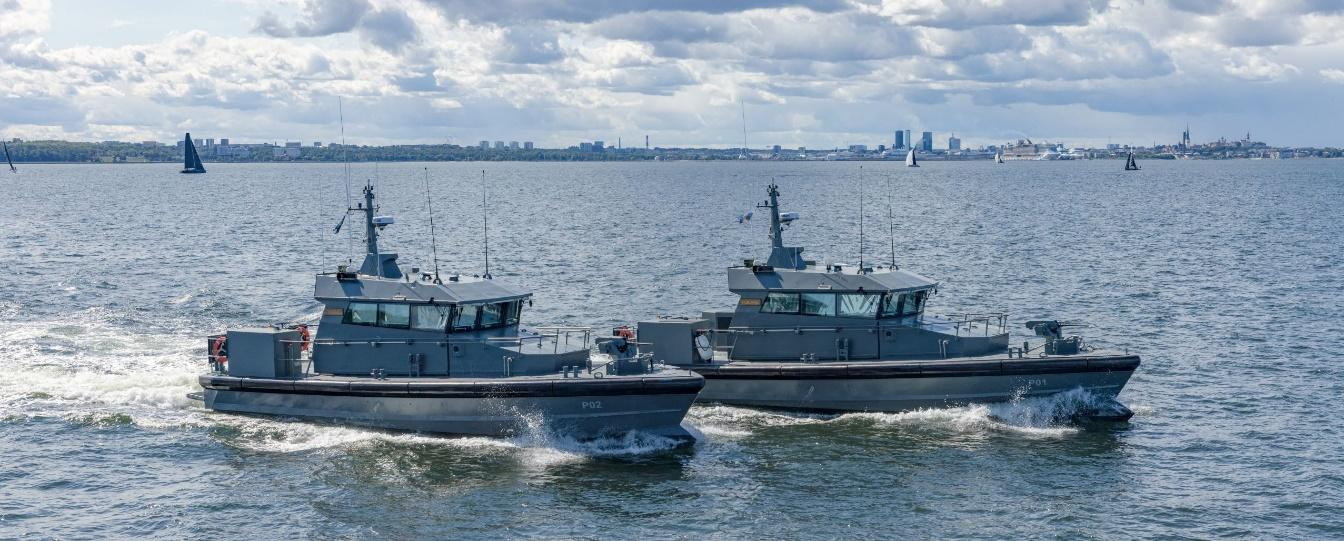
\includegraphics[width=6.10278in,height=2.45694in]{media/image3.jpg}

Joonis 1. Baltic Workboatsi patrullaevad Navy 18 WP \cite{ref12}

Käesoleva bakalaureusetöö eesmärgiks on arendada välja masinnägemise süsteem, mis abistab laeva käigukatsete läbiviimisel. See eeldab sobiliku riistvara, tarkvara ja masinõppe mudeli valimist, seejärel masinnägemise tarkvara loomist ja mudeli optimeerimist.

Püstitatud eesmärgi saavutamiseks otsitakse lahendust järgmistele probleemidele:

\begin{itemize}
\item
  Millist riistvara masinnägemise süsteemi jaoks kasutada?
\item
  Milline masinõppe mudel suudab merel objekte kõige paremini tuvastada?
\item
  Kuidas tuvastada objekte autonoomsel laeval, kasutades masinnägemist?
\item
  Kuidas optimeerida masinõppe mudelit piiratud ressursiga riistvara jaoks?
\end{itemize}

Lõputöö on üles ehitatud järgnevalt: Käigukatsete peatükis tutvustatakse laevade käigukatsete meetodit ning lahendust nende automatiseerimiseks. Peatükis 1 tuleb juttu masinnägemisest, selle olemusest ja tööpõhimõttest ning masinnägemisel kasutusel olevatest mudelitest selgitatakse spetsiifilisemalt konvolutsioonist närvivõrku. Peatükis 2 räägitakse riistvarast, mida masinnägemise süsteemi loomisel kasutatakse, riistvaraliselt spetsialiseeritud kiirenditest ja antakse süsteemi lihtsustatud ülevaade. Peatükis 3 kajastub ülevaade erinevatest masinnägemise rakenduse loomist võimaldavatest tarkvaradest ja selgitatakse välja millist masinnägemismudelit masinnägemise rakenduses kasutatakse. Peatükis 4 selgitatakse masinnägemise rakenduse olemust ja tööpõhimõtet, samuti kirjeldatakse selle arendusprotsessi ning optimeerimist. Peatükis 5 tehakse katseid masinnägemise mudelitega ja analüüsitakse kui palju mudelite optimeerimine mõjutab rakenduses kaadrite töötluse kiirust. Peatükk 6 võtab kokku töö sisu ning eesmärkide soorituse.
